\documentclass[12pt]{jarticle}
\usepackage{TUSIReport}
\usepackage{otf}
\usepackage[dvipdfmx]{graphicx}
\usepackage[dvipdfmx]{color}
\usepackage{amsmath}
\usepackage{amssymb}
\usepackage{color}
\usepackage{hhline}
\usepackage{fancybox,ascmac}
\usepackage{multirow}
\usepackage{url}
\usepackage{bm}
\usepackage{listings,jlisting}
\lstdefinestyle{log}{
    frame={tblr},
    basicstyle={\footnotesize},
    tabsize={4},
}
\lstdefinestyle{lsthtml}{
    language={html},
    backgroundcolor={\color[gray]{.85}},
    basicstyle={\small},
    identifierstyle={\small},
    commentstyle={\small\ttfamily \color[rgb]{0,0.5,0}},
    keywordstyle={\small\bfseries \color[rgb]{1,0,0}},
    ndkeywordstyle={\small},
    stringstyle={\small\ttfamily \color[rgb]{0,0,1}},
    frame={tb},
    breaklines=true,
    columns=[l]{fullflexible},
    numbers=left,
    xrightmargin=0zw,
    xleftmargin=3zw,
    numberstyle={\scriptsize},
    stepnumber=1,
    numbersep=1zw,
    morecomment=[l]{//}
}
\lstdefinestyle{lstcpp}{
    language={C++},
    backgroundcolor={\color[gray]{.85}},
    basicstyle={\small},
    identifierstyle={\small},
    commentstyle={\small\ttfamily \color[rgb]{0,0.5,0}},
    keywordstyle={\small\bfseries \color[rgb]{1,0,0}},
    ndkeywordstyle={\small},
    stringstyle={\small\ttfamily \color[rgb]{0,0,1}},
    frame={tb},
    breaklines=true,
    columns=[l]{fullflexible},
    numbers=left,
    xrightmargin=0zw,
    xleftmargin=3zw,
    numberstyle={\scriptsize},
    stepnumber=1,
    numbersep=1zw,
    morecomment=[l]{//}
}
\begin{document}
%%%%%%%%%%%%%%%%%%%%%%%%%%%%%%%%%%%%%%%%%%%%%%%%%%%%%%%%%%%%%%
% 表紙を出力する場合は,\提出者と\共同実験者をいれる
% \提出者{科目名}{課題名}{提出年}{提出月}{提出日}{学籍番号}{氏名}
% \共同実験者{一人目}{二人目}{..}{..}{..}{..}{..}{八人目}
%%%%%%%%%%%%%%%%%%%%%%%%%%%%%%%%%%%%%%%%%%%%%%%%%%%%%%%%%%%%%%
\提出者{情報工学実験2}{実験テーマ1 数理計画法}{2020}{10}{19}{4619055}{辰川力駆}
\共同実験者{}{}{}{}{}{}{}{}

%%%%%%%%%%%%%%%%%%%%%%%%%%%%%%%%%%%%%%%%%%%%%%%%%%%%%%%%%%%%%%
% 表紙を出力しない場合は,以下の「\表紙出力」をコメントアウトする
%%%%%%%%%%%%%%%%%%%%%%%%%%%%%%%%%%%%%%%%%%%%%%%%%%%%%%%%%%%%%%
\表紙出力

%%%%%%%%%%%%%%%%%%%%%%%%%%%%%%%%%%%%%%%%%%%%%%%%%%%%%%%%%%%%%%
% 以下はレポート本体である.別途 TeXファイルを作成し \input 使っても良い
%%%%%%%%%%%%%%%%%%%%%%%%%%%%%%%%%%%%%%%%%%%%%%%%%%%%%%%%%%%%%%

\section{実験の要旨}
本実験では実際に最適化問題を定式化をしながら解の検討をすることにより、
最適化問題への理解を深める。

\section{実験の目的}
最適化問題を解くための数理的手法は数理計画法と呼ばれる。
その数理計画法を現実問題に適用する際に役立つ基礎力を養うことを目的とする。

\section{実験の原理(理論)}
\subsection{用語の説明}
最適化問題は、数学的には、解集合と呼ばれる集合$S$と目的関数と呼ばれる関数
$f:S\rightarrow\boldsymbol{R}$が与えられたとき、
$f(\boldsymbol{x})$を最小にする$\boldsymbol{x}$
を求める問題であり、これを、
\begin{center}
    Minimize\ $f(\boldsymbol{x})$\ subject\ to\ $\boldsymbol{x}$\ $\in$\ $S$
\end{center}
とかく。
最適化問題の答え、つまり、
$\boldsymbol{S}$の任意の$\boldsymbol{x}$に対し、
$f(\boldsymbol{x^*})\leq f(\boldsymbol{x})$を満たす
$\boldsymbol{x^*}$を最適解と呼ぶ。
また、$\boldsymbol{x^*}$が局所的に最小なら、つまり、
\begin{equation}
    \exists \epsilon >0,\ \forall \boldsymbol{x} \in N_\epsilon(\boldsymbol{x^*}),\ f(\boldsymbol{x^*})\leq f(\boldsymbol{x})\nonumber
\end{equation}
が成り立つなら、
$\boldsymbol{x^*}$を局所的最適解と呼ぶ。
ただし、$N_\epsilon(\boldsymbol{x^*})=\{\boldsymbol{x};||\boldsymbol{x^*}-\boldsymbol{x}||<\epsilon\}$
である。
局所的最適解と区別するために最適解を大域的最適解と呼ぶことも多い。
大域的最適解は局所的最適解になっているが、逆は成り立たない。

\clearpage
\subsection{定式化の作り方}
定式化は、大雑把に言うと、言葉で説明された最適化問題に数式での表現を与えることである。
簡単な例を元に示す。

\subsubsection*{例1}
庭造り。長さ$10[m]$のフェンスがあり、このフェンスで囲われた長方形の庭を造りたいとする。
庭の面積を最大にするにはどうすれば良いか?
この例で制御できる数量は(値)は、庭の縦の長さ$x_1[m]$と横の長さ$x_2[m]$であり、
最適化問題の文脈では、
決定変数と呼ばれる。
また、決定変数が満たすべき条件は制約条件と呼ばれる。
まとめると、この問題は、$\boldsymbol{x}={}^t(x_1,x_2)$として、
\begin{eqnarray}
    f(\boldsymbol{x})=x_1x_2,\ S=\{\boldsymbol{x}; x_1,x_2\in \mathbb{R},\ x_1,x_2\geq 0,\ 2x_1+2x_2=10\} \nonumber
\end{eqnarray}
とすれば、「Maximize\ $f(\boldsymbol{x})$\ subject\ to\ $\boldsymbol{x}$\ $\in$\ $S$ 」とかける。


\subsubsection*{例2}
野菜ジュース。
栄養素$N_1,N_2,N_3$を補うために野菜$V_1$と$V_2$を使ったジュースを毎朝飲むことにした。
これらの野菜の評価と各要素の含有量は表1にまとめた。

また、栄養素$A_i$は一日に$b_i[mg]$だけ必要とする$(i=1,2,3)$。
費用を最小にするには各野菜をどれだけ購入すれば良いか?
ただし、野菜はグラム単位で購入できるものとする。

\begin{table}[htb]
    \begin{center}
        \caption{例2の各栄養素の含有量}
        \begin{tabular}{|c|c|c|c|c|}
            \hline
                      & 単価$[円/g]$ & 栄養素$A_1[mg/g]$ & 栄養素$A_2[mg/g]$ & 栄養素$A_3[mg/g]$ \\
            \hline
            野菜$V_1$ & $c_1$        & $a_{11}$          & $a_{12}$          & $a_{13}$          \\
            野菜$V_2$ & $c_2$        & $a_{21}$          & $a_{22}$          & $a_{23}$          \\
            \hline
        \end{tabular}
    \end{center}
\end{table}

例2の問題は、制御条件と目的関数が線形式で、
さらに、決定変数が連続値を取る連続変数となる最適化問題として定式化される。
このような問題は一般に線形計画問題と呼ばれる。

\clearpage
\subsubsection*{例3}
お菓子。
遠足に持っていくお菓子を300円の予算内で買いたい。
お菓子の候補として以下の5つまで絞った(「嬉しさ」は本人の主観)。

\begin{table}[htb]
    \begin{center}
        \caption{例3のお菓子の候補}
        \begin{tabular}{|c|c|c|c|c|c|}
            \hline
                     & 1:チョコ & 2:クッキー & 3:ポテチ & 4:グミ & 5:ガム \\
            \hline
            嬉しさ   & 10       & 5          & 7        & 6      & 3      \\
            価格[円] & 140      & 80         & 130      & 70     & 30     \\
            \hline
        \end{tabular}
    \end{center}
\end{table}
ただし、同じお菓子を2つ以上は買わないこととする。
この問題の定式化では決定変数は(連続値ではなく)離散値にするとうまくいくことがわかる。
具体的には、この問題は、
\begin{eqnarray}
    x_i=\left\{
    \begin{array}{l}
        1 i番目のお菓子を購入するとき \\
        0 i番目のお菓子を購入しないとき
    \end{array}
    \right. \nonumber
\end{eqnarray}
と解釈するものと約束し、$\boldsymbol{x}={}^t(x_1,x_2,x_3,x_4,x_5)$として、
\begin{eqnarray}
    f(\boldsymbol{x})&=&10x_1+5x_2+7x_3+6x_4+3x_5, \nonumber \\
    S&=&\{ \boldsymbol{x};x_1,x_2,x_3,x_4,x_5 \in \{0,1\},\ 140x_1+80x_2+130x_3+70x_4+30x_5\leq 300\}\nonumber
\end{eqnarray}
とすれば、「Maximize\ $f(\boldsymbol{x})$\ subject\ to\ $\boldsymbol{x}$\ $\in$\ $S$ 」とかける。



例3のように離散値をとる変数を整数変数、特に0か1の値をとる変数をバイナリ変数と呼ぶ。
バイナリ変数は「ON/OFF」や「取る/取らない」等を表現できる極めて有用な変数である。
整数変数を扱う最適化問題は整数最適化問題と呼ばれる。

整数変数と連続変数が混在する最適化問題はしばしば混合整数計画問題と呼ばれる。
以下の最後の例は、混合整数計画問題として定式化するのが自然な例である。

\subsubsection*{例4}
工場での生産計画。
ある工場で2つの製品$A_1$と$A_2$がそれぞれ機械$M_1$と$M_2$によって独立に製造されているとする。
機械$M_i$の生産効率は$e_i[kg/時間]$で、セットアップに$s_i[W]$と、
単位時間の稼働に$t_i[W/時間]$だけ電力を消費するとする($i=1,2$)。
一方、工場の1日の総消費電力の上限は$U^E[W]$で、また、
各機械の稼働時間の上限はともに$U^L$時間とする。
いま、製品$A_1$と$A_2$の単価がそれぞれ$p_1$と$p_2[万円/kg]$であるとすれば、
1日の総利益を最大にするには、
各機械の稼働時間をいくつに設定すればよいか?
ただし、機械を全く稼働させなければセットアップにかかる電力は生じないものとし、
製品$A_1$と$A_2$は(理想的であるが)製造した分だけ売れるものとする。

\clearpage

\section{実験方法}
次の各項目に取り組む。
\begin{itemize}
    \item[(1)] 最適化問題とみなせる現実問題の例を挙げる。
          ただし、目的関数、制約条件、決定変数を大雑把に述べる程度で良いものとする。
    \item[(2)]問1から問6に答えよ。
          \begin{itemize}
              \item[問1.] 例2の問題を定式化する。
              \item[問2.] 例2の定数に具体的な数値を適当に代入し、
                    そのときの最適解と最適値を求める。
                    ただし、$(x_1,x_2)$-平面を描いて制約条件を満たす解の領域を図示すること。
              \item[問3.] 例3の問題の最適解と最適値を求める。
              \item[問4.] 例3の定式化に以下の2つの制約条件を追加したいとする。
                    これらがどのように数式で表現できるかを述べ、その妥当性を説明する。
                    \begin{center}
                        \textbf{A}. グミとガムの両方は買わない\\
                        \textbf{B}. ポテチを買うならガムも買う\\
                    \end{center}
              \item[問5.] (例4の問題の定式化の準備)。
                    決定変数$x$と$y$を考える。
                    $x$はバイナリ変数、$y$は連続変数とする。
                    $x=1$のときに$y$は$a$以上$b$以下の値をとることができ、
                    $x=0$のときには$y=0$でないといけないようにしたい。
                    この制約条件を数式で表現し、その妥当性を説明する。
              \item[問6.] 例4の問題を定式化する。
          \end{itemize}

    \item[(3)]最適化問題とみなせる現実問題の例を挙げ、実際に定式化する。
          (1)の問題と同じでも良い。
\end{itemize}

\section{実験結果}

\subsection*{(1)}
現実の最適化問題として、1ルームのシェアハウスをすると考える。
長方形の部屋1つに対し、(2人分に分けるのはあまりにも容易なので)3人分に分けることを考える。
このとき仲が悪くならないように3つの面積の差が小さくなるように分ける。

例えば、$縦(H)\times 横(W)$(制約条件$1\leq H,W \leq 10^5$)のもとで3つに分けることを考えて
面積の最大値と最小値の差が最小になるように考えれば良い。

\clearpage
\subsection*{(2)}
\fbox{問1}
2つの野菜の合計の値段を$f(\boldsymbol{x})$とし、
2つの野菜($V_1$,$V_2$)の量をそれぞれ$x_1[g]$と$x_2[g]$とする。
2つの野菜の単価と取れる栄養素は表1の通りである。
栄養素$A_i$は1日に$b_i[mg]$取らなければならない。
これらを定式化すると、
\begin{eqnarray}
    f(\boldsymbol{x})=c_1 x_1 +c_2 x_2,\ S=\{\boldsymbol{x};x_1,x_2\in \mathbb{R},\ x_1,x_2\geq 0,\ a_{1i} x_1+a_{2i}x_2\geq b_i(i=1,2,3)\}\nonumber
\end{eqnarray}
とすれば、「Minimize\ $f(\boldsymbol{x})$\ subject\ to \ $\boldsymbol{x}$\ $\in$ $S$\ 」とかける。

\fbox{問2}
表1の例として具体的な数値を適当に代入したものを表3に示す。
\begin{table}[htb]
    \begin{center}
        \caption{例2の各栄養素の含有量(具体的な例)}
        \begin{tabular}{|c|c|c|c|c|}
            \hline
                      & 単価$[円/g]$ & 栄養素$A_1[mg/g]$ & 栄養素$A_2[mg/g]$ & 栄養素$A_3[mg/g]$ \\
            \hline
            野菜$V_1$ & 3            & 120               & 80                & 30                \\
            野菜$V_2$ & 2.5          & 100               & 90                & 20                \\
            \hline
        \end{tabular}
    \end{center}
\end{table}

また、$(b_1,b_2,b_3)=(10000,15000,5000)$とする。
横軸が$x_1$,縦軸が$x_2$とすると、実行可能領域は図1の黒の斜線部分となる。
ただし、境界を含む。
\begin{figure}[h]
    \begin{center}
        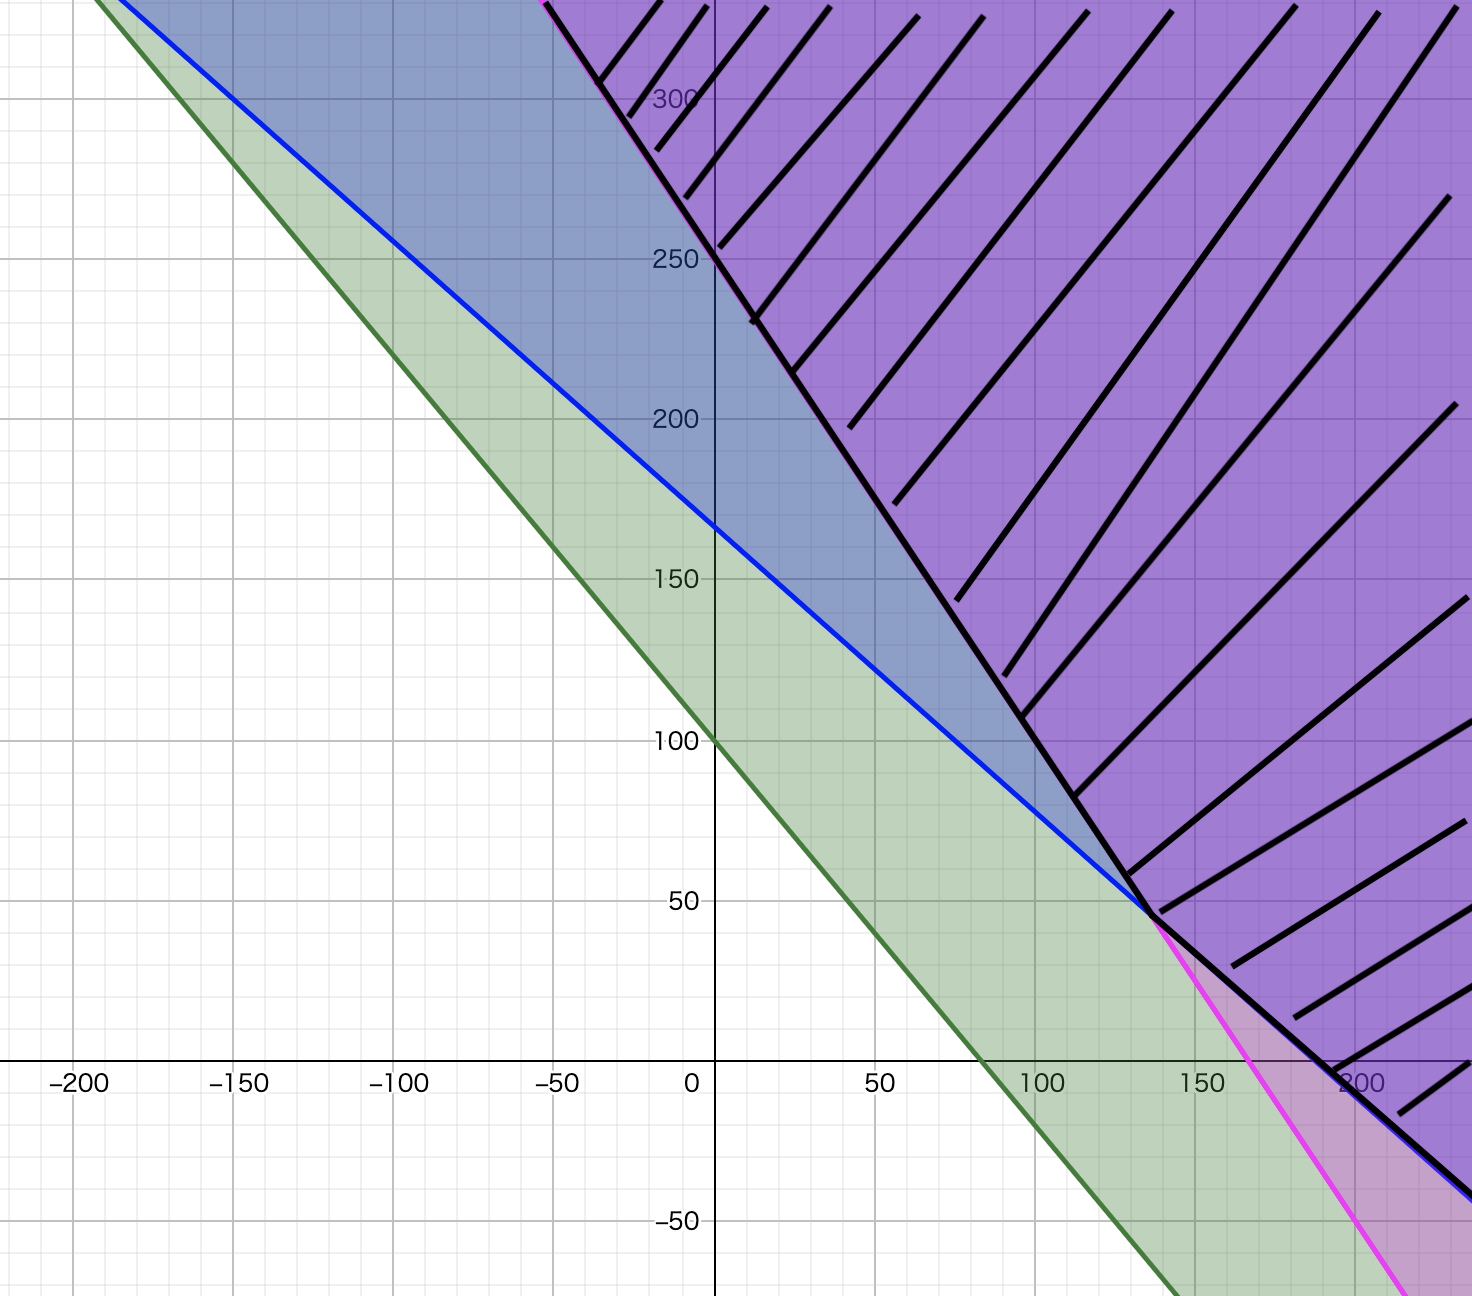
\includegraphics[scale=0.2]{kadai1_1.png}
    \end{center}
    \caption{問2の実行可能領域}
\end{figure}

よって、$f(\boldsymbol{x})=3x_1+2.5x_2$を最小にすることを考えると、
最適解は$(x_1,x_2)\approx (136.364,45.455)$で、
最適値は523円である。

\clearpage
\fbox{問3}
この問題は一般に個数制限ありナップサック問題と言われ、動的計画法で解くことができる。

まず、$x_1からx_5$を価格の大きい順に並べ替える。
そうすると価格が大きい順に$x_1,x_3,x_2,x_4,x_5$となる。
そして、$x_1$だけ買えるとき、最適解はどれかを考える。
次に$x_1,x_3$が買えるときに最適解はどれかを考える。
このように1つずつ買えるのを増やして考える。

これを分かりやすくしたのが表4である。
縦は1つずつ増やすお菓子(価格が高い順)であり、横は予算額である。
そして、表の内の値は嬉しさの最大値である。
\begin{table}[htb]
    \begin{center}
        \caption{問3の動的計画法の表}
        \begin{tabular}{|c|c|c|c|c|c|c|c|c|c|c|c|c|c|c|}
            \hline
                  & 30  & 40  & 50  & 60  & 70  & 80  & 90  & 100 & 110 & 120 & 130 & 140 & 150 & 160 \\
            \hline
            $x_1$ & 0   & 0   & 0   & 0   & 0   & 0   & 0   & 0   & 0   & 0   & 0   & 10  & 10  & 10  \\ \hline
            $x_3$ & 0   & 0   & 0   & 0   & 0   & 0   & 0   & 0   & 0   & 0   & 7   & 10  & 10  & 10  \\ \hline
            $x_2$ & 0   & 0   & 0   & 0   & 0   & 5   & 5   & 5   & 5   & 5   & 7   & 10  & 10  & 10  \\ \hline
            $x_4$ & 0   & 0   & 0   & 0   & 6   & 6   & 6   & 6   & 6   & 6   & 7   & 10  & 11  & 11  \\ \hline
            $x_5$ & 3   & 3   & 3   & 3   & 6   & 6   & 6   & 9   & 9   & 9   & 9   & 10  & 11  & 11  \\
            \hline
            \hline
                  & 170 & 180 & 190 & 200 & 210 & 220 & 230 & 240 & 250 & 260 & 270 & 280 & 290 & 300 \\
            \hline
            $x_1$ & 10  & 10  & 10  & 10  & 10  & 10  & 10  & 10  & 10  & 10  & 10  & 10  & 10  & 10  \\ \hline
            $x_3$ & 10  & 10  & 10  & 10  & 10  & 10  & 10  & 10  & 10  & 10  & 17  & 17  & 17  & 17  \\ \hline
            $x_2$ & 10  & 10  & 10  & 10  & 12  & 15  & 15  & 15  & 15  & 15  & 17  & 17  & 17  & 17  \\ \hline
            $x_4$ & 11  & 11  & 11  & 13  & 16  & 16  & 16  & 16  & 16  & 16  & 17  & 18  & 21  & 21  \\ \hline
            $x_5$ & 13  & 14  & 14  & 14  & 16  & 16  & 16  & 19  & 19  & 19  & 19  & 19  & 21  & 21  \\
            \hline
        \end{tabular}
    \end{center}
\end{table}

したがって、表より最適解は$(x_1,x_2,x_3,x_4,x_5)=(1,1,0,1,0)$つまり、チョコとクッキーとグミを買ったときで、
最適値(嬉しさ)は21である。

\fbox{問4}

\textbf{Aについて}

グミとガムについてなので$x_4$,$x_5$についての制約条件を考えれば良い。
数式で表現すると、
\begin{eqnarray}
    x_4+x_5<2\nonumber
\end{eqnarray}
と表せる。
実際、グミとガムを両方買う時のみ$x_4+x_5=2$となり、
片方のみ買う時は$x_4+x_5=1$で両方買わない時は$x_4+x_5=0$なので、
妥当性に欠けていないことがわかる。

\textbf{Bについて}

ポテチとガムについてなので$x_3$,$x_5$についての制約条件を考えれば良い。
数式で表現すると、
\begin{eqnarray}
    x_3\leq x_5\nonumber
\end{eqnarray}
と表せる。
実際、ポテチを買う時は$1\leq x_5$となり、$x_5=1$つまりガムを買わないといけなくなる。
また、ポテチを買わない時は$0 \leq x_5$となり、$x_5=0,1$の両方をとるのでどちらでも良くなる。
よって、妥当性に欠けていないことがわかる。

\clearpage

\fbox{問5}
この制約条件を数式で表現すると、
\begin{eqnarray}
    ax\leq y \leq bx,\ x\in \{0,1\}\nonumber
\end{eqnarray}
となる。
実際、$x=0$のとき、$0\leq y \leq 0$、つまり$y=0$となる。
また、$x=1$のとき、$a\leq y \leq b$となり、妥当性に欠けていないことがわかる。

\fbox{問6}
各機械に対して、稼働しているかしていないかという変数をバイナリ変数$(x_1,x_2)$、
稼働時間を連続変数を用いて
\begin{eqnarray}
    \boldsymbol{y}={}^t(y_1,y_2) \nonumber
\end{eqnarray}
として、問題を定式化すると、
\begin{eqnarray}
    f(\boldsymbol{y})&=&p_1e_1y_1+p_2e_2y_2\nonumber \\
    S&=&\{\boldsymbol{y}; y_1,y_2 \in \mathbb{R},\ x_1,x_2\in \{0,1\},\ 0 \leq y_1,y_2 \leq U^L,\ 0 \leq (s_1+t_1y_1)x_1+(s_2+t_2y_2)x_2\leq U^E\} \nonumber
\end{eqnarray}
とすれば、「Maximize\ $f(\boldsymbol{y})$ subject to\ $\boldsymbol{y}$\ $\in$\ $S$ 」とかける。

\subsection*{(3)}
(1)と同様にシェアハウスの問題を考える。
長方形の部屋1つ$縦(H)\times 横(W)$($1\leq H,W \leq 10^5$)に対し、3人分に分けることを考える。
ただし、面積の差が小さくなるようにする。
3人に分けられる面積を
\begin{eqnarray}
    \boldsymbol{x}={}^t(x_1,x_2,x_3) \nonumber
\end{eqnarray}
として、問題を定式化すると、
\begin{eqnarray}
    f(\boldsymbol{x})&=& \text{max}\{x_1,x_2,x_3\}-\text{min}\{x_1,x_2,x_3\} \nonumber\\
    S&=&\{\boldsymbol{x};x_1,x_2,x_3 \in \mathbb{R},\ 1\leq H,W \leq 10^5,\ x_1+x_2+x_3=HW\} \nonumber
\end{eqnarray}
とすれば、「Minimize\ $f(\boldsymbol{x})$ subject to\ $\boldsymbol{x}$\ $\in$\ $S$ 」とかける。

\subsubsection*{[発展]}
(3)の問題を解いてみる。
c++のソースコード(saiteki.cpp)を付録に載せた。
例えば、入力$(H,W)=(30,5)$に対しての最適値は0となる。
また、入力$(H,W)=(79,67)$に対しての最適値は60となる。
求める考え方は考察で述べる。

\clearpage
\section{検討・考察}
\subsection*{(2)}
\fbox{問1}

\fbox{問2}

\fbox{問3}
実験結果では動的計画法で解いたが、今回は5つお菓子しかなかったので、$2^5=32$通りを探索するという考えでも解くことができる。
ただし、数が多くなると全探索をするのに時間がかかってしまうので、
その場合は自分が行ったような動的計画法などの違う方法で求めるべきである。

\fbox{問4}

\fbox{問5}

\fbox{問6}

\subsection*{(3)}

\section{まとめ}


\clearpage

% 参考文献
\begin{thebibliography}{99}
    \label{sannkoubunnkenn_chapter}
    \bibitem[1]{rikadai}東京理科大学工学部情報工学科 情報工学実験2 2020年度
    東京理科大学工学部情報工学科出版

    \bibitem[2]{toukei}
    関数グラフ - GeoGebra

    \url{https://www.geogebra.org/graphing?lang=ja}

    最終閲覧日2020/10/23

\end{thebibliography}


\clearpage

% 付録
\appendix
\section{付録}
\begin{lstlisting}[style = lstcpp,caption=saiteki.cpp]
    #include <bits/stdc++.h>
    using namespace std;
    template <class T>
    inline bool chmax(T &a, T b)
    {
        if (a < b)
        {
            a = b;
            return 1;
        }
        return 0;
    }
    template <class T>
    inline bool chmin(T &a, T b)
    {
        if (a > b)
        {
            a = b;
            return 1;
        }
        return 0;
    }
    
    using pll = pair<long long, long long>;
    pll sub(long long h, long long w)
    {
        if (h % 2 == 0 || w % 2 == 0)
            return {h * w / 2, h * w / 2};
        if (h > w)
            swap(h, w);
        return {h * (w + 1) / 2, h * (w - 1) / 2};
    }
    
    int main()
    {
        long long H, W;
        cin >> H >> W;
        long long res = H * W;
    
        for (long long h = 1; h < H; ++h)
        {
            vector<long long> a(3);
            a[0] = h * W;
            auto p = sub(H - h, W);
            a[1] = p.first, a[2] = p.second;
            sort(a.begin(), a.end());
            chmin(res, a.back() - a[0]);
        }
        for (long long w = 1; w < W; ++w)
        {
            vector<long long> a(3);
            a[0] = H * w;
            auto p = sub(H, W - w);
            a[1] = p.first, a[2] = p.second;
            sort(a.begin(), a.end());
            chmin(res, a.back() - a[0]);
        }
        cout << res << endl;
    }
\end{lstlisting}


%%%%%%%%%%%%%%%%%%%%%%%%%%%%%%%%%%%%%%%%%%%%%%%%%%%%%%%%%%%%%%
\end{document}